\documentclass{IEEEtran}
\usepackage{cite}
\usepackage{amsmath,amssymb,amsfonts}
\usepackage{algorithmic}
\usepackage{graphicx}
\usepackage{pgfplots}
\usepackage{tikz}
\usepackage{textcomp}
\usepackage{booktabs}
\usepackage{listings}
\usepackage{xcolor} % for setting colors
\definecolor{vblue}{RGB}{49,49,255}
\definecolor{vgreen}{RGB}{104,180,104}

\usepackage {tikz}
\usetikzlibrary {positioning}
%\usepackage {xcolor}
\definecolor {processblue}{cmyk}{0.96,0,0,0}

\definecolor{light-gray}{gray}{0.95} %the shade of grey that stack exchange uses
% set the default code style
\lstset{
	basicstyle=\ttfamily,  
	backgroundcolor=\color{light-gray}
}
 \lstdefinestyle{cpp}{
 	language=C++,
 	basicstyle=\small\ttfamily,
 	keywordstyle=\color{vblue},
 	identifierstyle=\color{black},
 	commentstyle=\color{vgreen},
 	numberstyle=\tiny\color{black},
 	numbersep=10pt,
 	tabsize=4,
 	moredelim=*[s][\colorIndex]{[}{]},
 	literate=*{:}{:}1
 }

\def\BibTeX{{\rm B\kern-.05em{\sc i\kern-.025em b}\kern-.08em
		T\kern-.1667em\lower.7ex\hbox{E}\kern-.125emX}}
\begin{document}
\title{Parallel Congruence Closure SAT solver}
\author{Enrico Martini, VR445204}
\maketitle
\begin{abstract}
 In this report is presented a parallel implementation of a congruence closure algorithm for deduction in ground equational theories, able to solve a set of clauses in the quantifiers free fragment of first order logic, based on equality among variables, constants, function applications, recursive data structures with their elements and elements of arrays.
\end{abstract}
\section{Introduction}
The first theory considered is the class of SMT problems is called EUF (Equality with Uninterpreted Functions), containing atoms that are equalities between terms built over uninterpreted function symbols. EUF (i.e., SAT modulo the theory of congruences) is important in applications such as the verification of pipelined processors, where, if the control is verified, the concrete data operations can be abstracted by uninterpreted function symbols.\cite{NIEUWENHUIS2007557} It is the most important theory because its congruence closure algorithm is the core of the entire solver. The implemented algorithm also integrates the theory of lists $\mathcal{T}_{cons}$. 
\section{Methodology}


\subsection{Algorithm}
The most interesting feature of this implementation is the organization of the information within the data structures, shaped to be efficient.
\begin{lstlisting}[style=cpp]
class Node{
private:
	std::string 				fn;                  
	uint_fast16_t 				id;                
	std::vector<uint_fast16_t> 	args; 
	uint_fast16_t 				find;              
	std::vector<uint_fast16_t> 	ccpar;
};
\end{lstlisting}
The type used to represents indexes is \verb|uint_fast16_t|, that is the fastest available unsigned integer with at least 16 bits.


\subsection{Equality theory congruence closure example}
\begin{align*}
	\mathcal{F} : x = y \land f(x) \ne f(y)
\end{align*}

\begin{lstlisting}
x=y&f(x)!=f(y)
\end{lstlisting}

\begin {center}
\resizebox{3.5cm}{!}{
\begin {tikzpicture}[-latex ,auto ,node distance =2 cm and 2cm ,on grid ,
semithick ,
state/.style ={ circle ,top color =white , bottom color = white ,
	draw,black , text=black , minimum width =0.5 cm}]
\node[state] (N0) {0 : x};
\node[state] (N1) [right=of N0]{1 : y};
\node[state] (N2) [above =of N0]{2 : f};
\node[state] (N3) [above right=of N0] {3 : f};
\path (N2) edge [above] node[left] {} (N0);
\path (N3) edge [above] node[left] {} (N1);
\end{tikzpicture}
}
\end{center}

\begin{lstlisting}
node		find		ccpar
________________________________________
0x		0		2
1y		1		3
2f->0		2		-
3f->1		3		-
\end{lstlisting}

\begin{lstlisting}
MERGE 0 1
UNION 0 1
MERGE 2 3 ?
CONGRUENT 2 3 = 1
\end{lstlisting}


\begin {center}
\resizebox{3.5cm}{!}{
	\begin {tikzpicture}[-latex ,auto ,node distance =2 cm and 2cm ,on grid ,
	semithick ,
	state/.style ={ circle ,top color =white , bottom color = white ,
		draw,black , text=black , minimum width =0.5 cm}]
	\node[state] (N0) {0 : x};
	\node[state] (N1) [right=of N0]{1 : y};
	\node[state] (N2) [above =of N0]{2 : f};
	\node[state] (N3) [above right=of N0] {3 : f};
	\path (N2) edge [above] node[left] {} (N0);
	\path (N3) edge [above] node[left] {} (N0);
	\path (N0) edge[,-,densely dotted] [above] node[left] {} (N1);
\end{tikzpicture}
}
\end{center}

\begin{lstlisting}
node		find		ccpar
________________________________________
0x		0		23
1y		0		-
2f->0		2		-
3f->1		3		-
\end{lstlisting}

\begin{lstlisting}
MERGE 2 3
UNION 2 3
\end{lstlisting}

\begin {center}
\resizebox{3.5cm}{!}{
	\begin {tikzpicture}[-latex ,auto ,node distance =2 cm and 2cm ,on grid ,
	semithick ,
	state/.style ={ circle ,top color =white , bottom color = white ,
		draw,black , text=black , minimum width =0.5 cm}]
	\node[state] (N0) {0 : x};
	\node[state] (N1) [right=of N0]{1 : y};
	\node[state] (N2) [above =of N0]{2 : f};
	\node[state] (N3) [above right=of N0] {3 : f};
	\path (N2) edge [above] node[left] {} (N0);
	\path (N3) edge [above] node[left] {} (N0);
	\path (N0) edge[,-,densely dotted] [above] node[left] {} (N1);		\path (N2) edge[,-,densely dotted] [above] node[left] {} (N3);
\end{tikzpicture}
}
\end{center}

\begin{lstlisting}
node		find		ccpar
________________________________________
0x		0		23
1y		0		-
2f->0		2		-
3f->1		2		-
\end{lstlisting}

\begin {center}
\resizebox{3.5cm}{!}{
	\begin {tikzpicture}[-latex ,auto ,node distance =2 cm and 2cm ,on grid ,
	semithick ,
	state/.style ={ circle ,top color =white , bottom color = white ,
		draw,black , text=black , minimum width =0.5 cm}]
	\node[state] (N0) {0 : x};
	\node[state] (N1) [right=of N0]{1 : y};
	\node[state] (N2) [above =of N0]{2 : f};
	\node[state] (N3) [above right=of N0] {3 : f};
	\path (N2) edge [above] node[left] {} (N0);
	\path (N3) edge [above] node[left] {} (N0);
	\path (N0) edge[,-,densely dotted] [above] node[left] {} (N1);		\path (N2) edge[,-,red] [above] node[left] {} (N3);
\end{tikzpicture}
}
\end{center}

\begin{lstlisting}
UNSAT
\end{lstlisting}

\subsection{List theory congruence closure example}

\begin{align*}
\mathcal{F} : cons(car(x),cdr(x)) = x \land atom(x) 
\end{align*}

\begin{lstlisting}
atom(x)&cons(car(x),cdr(x))=x
\end{lstlisting}


\begin {center}
\resizebox{4.5cm}{!}{
	\begin {tikzpicture}[-latex ,auto ,node distance =2 cm and 2cm ,on grid ,
	semithick ,
	state/.style ={ circle ,top color =white , bottom color = white ,
		draw,black , text=black , minimum width =0.5 cm}]
	\node[state] (N0) {0 : x};
	\node[state] (N1) [above left=of N0]{1 : car};
	\node[state] (N2) [above right=of N0]{2 : cdr};
	\node[state] (N3) [above right =of N1] {3 : cons};
	\node[state] (N4) [above left=of N3]{4 : car};
	\node[state] (N5) [above right=of N3]{5 : cdr};
	\path (N1) edge [above] node[left] {} (N0);
	\path (N2) edge [above] node[left] {} (N0);
	\path (N3) edge [above] node[left] {} (N1);
	\path (N3) edge [above] node[left] {} (N2);
	\path (N4) edge [above] node[left] {} (N3);
	\path (N5) edge [above] node[left] {} (N3);
\end{tikzpicture}
}
\end{center}


\begin{lstlisting}
MERGE 4 1
UNION 4 1
MERGE 5 2
UNION 5 2
\end{lstlisting}

\begin {center}
\resizebox{4.5cm}{!}{
	\begin {tikzpicture}[-latex ,auto ,node distance =2 cm and 2cm ,on grid ,
	semithick ,
	state/.style ={ circle ,top color =white , bottom color = white ,
		draw,black , text=black , minimum width =0.5 cm}]
	\node[state] (N0) {0 : x};
	\node[state] (N1) [above left=of N0]{1 : car};
	\node[state] (N2) [above right=of N0]{2 : cdr};
	\node[state] (N3) [above right =of N1] {3 : cons};
	\node[state] (N4) [above left=of N3]{4 : car};
	\node[state] (N5) [above right=of N3]{5 : cdr};
	\path (N1) edge [above] node[left] {} (N0);
	\path (N2) edge [above] node[left] {} (N0);
	\path (N3) edge [above] node[left] {} (N1);
	\path (N3) edge [above] node[left] {} (N2);
	\path (N4) edge [above] node[left] {} (N3);
	\path (N5) edge [above] node[left] {} (N3);
	\path (N2) edge[,-,densely dotted] [above] node[left] {} (N5);
	\path (N1) edge[,-,densely dotted] [above] node[left] {} (N4);
\end{tikzpicture}
}
\end{center}

\begin{lstlisting}
node		find		ccpar
________________________________________
0x		0		12
1car->0		4		-
2cdr->0		5		-
3cons->12	3		45
4car->3		4		3
5cdr->3		5		3
\end{lstlisting}



\begin{lstlisting}
MERGE 3 0
UNION 3 0
MERGE 4 1 ?
MERGE 4 2 ?
CONGRUENT 4 2 = 0
MERGE 5 1 ?
CONGRUENT 5 1 = 0
MERGE 5 2 ?
\end{lstlisting}

\begin {center}
\resizebox{4.5cm}{!}{
	\begin {tikzpicture}[-latex ,auto ,node distance =2 cm and 2cm ,on grid ,
	semithick ,
	state/.style ={ circle ,top color =white , bottom color = white ,
		draw,black , text=black , minimum width =0.5 cm}]
	\node[state] (N0) {0 : x};
	\node[state] (N1) [above left=of N0]{1 : car};
	\node[state] (N2) [above right=of N0]{2 : cdr};
	\node[state] (N3) [above right =of N1] {3 : cons};
	\node[state] (N4) [above left=of N3]{4 : car};
	\node[state] (N5) [above right=of N3]{5 : cdr};
	\path (N1) edge [above] node[left] {} (N0);
	\path (N2) edge [above] node[left] {} (N0);
	\path (N3) edge [above] node[left] {} (N1);
	\path (N3) edge [above] node[left] {} (N2);
	\path (N4) edge [above] node[left] {} (N3);
	\path (N5) edge [above] node[left] {} (N3);
	\path (N2) edge[,-,densely dotted] [above] node[left] {} (N5);
	\path (N1) edge[,-,densely dotted] [above] node[left] {} (N4);
	\path (N3) edge[,-,densely dotted] [above] node[left] {} (N0);
\end{tikzpicture}
}
\end{center}

\begin{lstlisting}
node		find		ccpar
________________________________________
0x		3		-
1car->0		4		-
2cdr->0		5		-
3cons->12	3		4512
4car->3		4		3
5cdr->3		5		3
\end{lstlisting}
\begin {center}
\resizebox{4.5cm}{!}{
	\begin {tikzpicture}[-latex ,auto ,node distance =2 cm and 2cm ,on grid ,
	semithick ,
	state/.style ={ circle ,top color =white , bottom color = white ,
		draw,black , text=black , minimum width =0.5 cm}]
	\node[state] (N0) {0 : x};
	\node[state] (N1) [above left=of N0]{1 : car};
	\node[state] (N2) [above right=of N0]{2 : cdr};
	\node[state] (N3) [above right =of N1] {3 : cons};
	\node[state] (N4) [above left=of N3]{4 : car};
	\node[state] (N5) [above right=of N3]{5 : cdr};
	\path (N1) edge [red,above] node[left] {} (N0);
	\path (N2) edge [red,above] node[left] {} (N0);
	\path (N3) edge [above] node[left] {} (N1);
	\path (N3) edge [above] node[left] {} (N2);
	\path (N4) edge [above] node[left] {} (N3);
	\path (N5) edge [above] node[left] {} (N3);
	\path (N2) edge[,-,densely dotted] [above] node[left] {} (N5);
	\path (N1) edge[,-,densely dotted] [above] node[left] {} (N4);
	\path (N3) edge[,-,densely dotted] [above] node[left] {} (N0);
\end{tikzpicture}
}
\end{center}
\begin{lstlisting}
Euality theory passed
UNSAT
\end{lstlisting}


\subsection{Array theory congruence closure example}

\begin{align*}
\mathcal{F} : e=select(store(a,i,e),j) \land select(a,j) \ne e
\end{align*}

\begin{lstlisting}
e=select(store(a,i,e),j)&select(a,j)!=e
\end{lstlisting}

\begin{lstlisting}
detected store
\end{lstlisting}

\begin{align*}
&\mathcal{F}_1 : e=e \land j=i \land select(a,j) \ne e\\
&\mathcal{F}_2 : e=select(a,j) \land j \ne i \land select(a,j) \ne e
\end{align*}


\begin{lstlisting}
1: e=e&j=i&select(a,j)!=e
2: e=select(a,j)&j!=i&select(a,j)!=e
\end{lstlisting}


\begin {center}
\resizebox{7.5cm}{!}{
	\begin {tikzpicture}[-latex ,auto ,node distance =2cm and 2cm ,on grid ,
	semithick ,
	state/.style ={ circle ,top color =white , bottom color = white ,
		draw,black , text=black , minimum width =0.5 cm}]
	\node[state] (N0) {0 : e};
	\node[state] (N1) [right=of N0]{1 : j};
	\node[state] (N2) [right=of N1]{2 : i};
	\node[state] (N3) [right =of N2] {3 : a};
	\node[state] (N4) [above left=of N3]{4 : select};
	\path (N4) edge [above] node[left] {} (N3);
	\path (N4) edge [above] node[left] {} (N1);
\end{tikzpicture}
}
\end{center}

\begin{lstlisting}
node		find		ccpar
________________________________________
0e		0		-
1j		1		4
2i		2		-
3a		3		4
4select->31	4		-
\end{lstlisting}
\begin{lstlisting}
MERGE 0 0
MERGE 1 2
UNION 1 2
\end{lstlisting}

\begin {center}
\resizebox{7.5cm}{!}{
	\begin {tikzpicture}[-latex ,auto ,node distance =2 cm and 2cm ,on grid ,
	semithick ,
	state/.style ={ circle ,top color =white , bottom color = white ,
		draw,black , text=black , minimum width =0.5 cm}]
	\node[state] (N0) {0 : e};
	\node[state] (N1) [right=of N0]{1 : j};
	\node[state] (N2) [right=of N1]{2 : i};
	\node[state] (N3) [right =of N2] {3 : a};
	\node[state] (N4) [above left=of N3]{4 : select};
	\path (N4) edge [above] node[left] {} (N3);
	\path (N4) edge [above] node[left] {} (N1);
	\path (N1) edge[,-,densely dotted] [above] node[left] {} (N2);
\end{tikzpicture}
}
\end{center}

\begin{lstlisting}
node		find		ccpar
________________________________________
0e		0		-
1j		1		4
2i		1		-
3a		3		4
4select->31	4		-
\end{lstlisting}

\begin {center}
\resizebox{7.5cm}{!}{
	\begin {tikzpicture}[-latex ,auto ,node distance =2 cm and 2cm ,on grid ,
	semithick ,
	state/.style ={ circle ,top color =white , bottom color = white ,
		draw,black , text=black , minimum width =0.5 cm}]
	\node[state] (N0) {0 : e};
	\node[state] (N1) [blue,right=of N0]{1 : j};
	\node[state] (N2) [blue,right=of N1]{2 : i};
	\node[state] (N3) [blue,right =of N2] {3 : a};
	\node[state] (N4) [blue,above left=of N3]{4 : select};
	\path (N4) edge [blue,above] node[left] {} (N3);
	\path (N4) edge [blue,above] node[left] {} (N1);
	\path (N1) edge[blue,-,densely dotted] [above] node[left] {} (N2);
\end{tikzpicture}
}
\end{center}

\begin{lstlisting}
Euality theory passed
SAT
\end{lstlisting}


\section{Validation}


\section{Benchmarks}
\begin{table}[htpb]
	\centering
	\caption{Performance results with simple algorithm.}
	\label{tab:norm}
	\resizebox{\columnwidth}{!}{%
	\begin{tabular}{|c|l|r|r|r|}
		\hline
		\textbf{Test} & \textbf{\#Formulas} & \textbf{Sequential (s)} & \textbf{Parallel (s)} & \textbf{Speedup} \\ \hline
		7             & 128                 & 0,0117                  & 0,0001                & 82,1             \\ \hline
		8             & 256                 & 0,0290                  & 0,0003                & 100,1            \\ \hline
		9             & 512                 & 0,0612                  & 0,0008                & 78,8             \\ \hline
		10            & 1024                & 0,1374                  & 0,0026                & 52,1             \\ \hline
		11            & 2048                & 0,2988                  & 0,0103                & 29,1             \\ \hline
		12            & 4096                & 0,6736                  & 0,0442                & 15,3             \\ \hline
		13            & 8192                & 1,5526                  & 0,1968                & 7,9              \\ \hline
		14            & 16384               & 3,7465                  & 1,6690                & 2,2              \\ \hline
		15            & 32768               & 13,8530                 & 9,5786                & 1,4              \\ \hline
	\end{tabular}
	}
\end{table}

% Please add the following required packages to your document preamble:
% \usepackage{graphicx}
\begin{table}[htpb]
	\centering
	\caption{Performance results with use of forbidden list}
	\label{tab:fl}
	\resizebox{\columnwidth}{!}{%
		\begin{tabular}{|c|l|r|r|r|}
			\hline
			\textbf{Test} & \textbf{\#Formulas} & \textbf{Sequential (s)} & \textbf{Parallel (s)} & \textbf{Speedup} \\ \hline
			7             & 128                 & 0,0128              & 0,0001            & 97,3             \\ \hline
			8             & 256                 & 0,0273              & 0,0003            & 107,6            \\ \hline
			9             & 512                 & 0,0605              & 0,0007            & 88,6             \\ \hline
			10            & 1024                & 0,1341              & 0,0024            & 57,0             \\ \hline
			11            & 2048                & 0,2964              & 0,0099            & 29,9             \\ \hline
			12            & 4096                & 0,6639              & 0,0430            & 15,5             \\ \hline
			13            & 8192                & 1,5309              & 0,1854            & 8,3              \\ \hline
			14            & 16384               & 3,7426              & 1,7264            & 2,2              \\ \hline
			15            & 32768               & 13,8145             & 9,4844            & 1,5              \\ \hline
		\end{tabular}%
	}
\end{table}

\section{Performance Analysis}



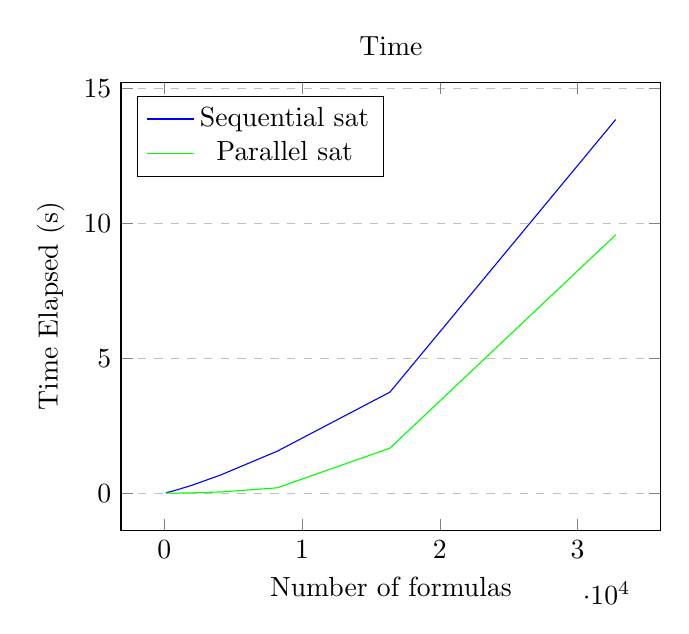
\begin{tikzpicture}
\begin{axis}[
title={Time},
ylabel={Time Elapsed (s)},
xlabel={Number of formulas},
legend pos=north west,
ymajorgrids=true,
grid style=dashed,
]

\addplot[color=blue]
coordinates {
	(128,0.0117)(256,0.0290)(512,0.0612)(1024,0.1374)(2048,0.2988)(4096,0.6736)(8192,1.5526)(16384,3.7465)(32768,13.8530)
};
\addplot[color=green]
coordinates {
	(128,0.0001)(256,0.0003)(512,0.0008)(1024,0.0026)(2048,0.0103)(4096,0.0442)(8192,0.1968)(16384,1.6690)(32768,9.5786)
};

\legend{Sequential sat,Parallel sat}

\end{axis}
\end{tikzpicture}

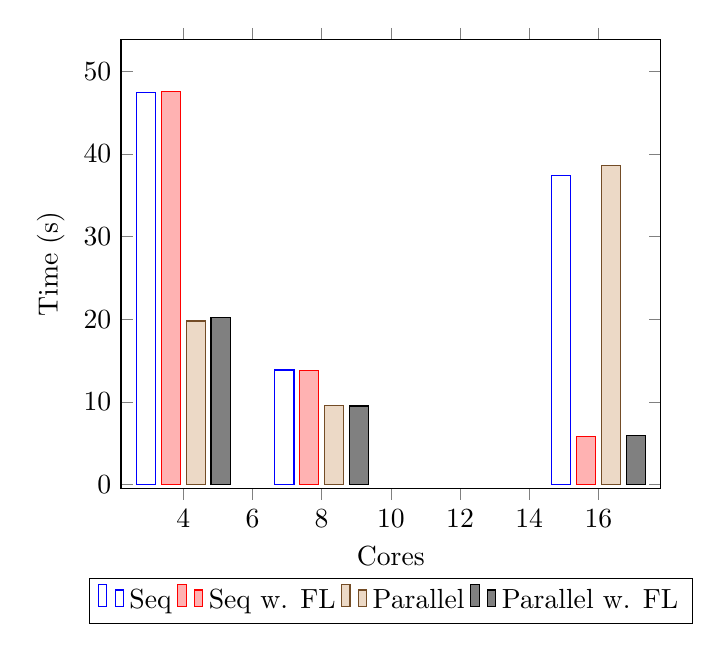
\begin{tikzpicture}
\begin{axis}[
x tick label style={
	/pgf/number format/1000 sep=},
ylabel=Time (s),
enlargelimits=0.15,
legend style={at={(0.5,-0.2)},
	anchor=north,legend columns=-1},
ybar,
bar width=7pt,
xlabel=Cores\\
]
\addplot[color=blue,domain=15:15]
coordinates {(4,47.4944)(8,13.8530)(16,37.3613)};
\addplot 
coordinates {(4,47.5747)(8,13.8145)(16,5.8145)};
\addplot 
coordinates {(4,19.7812)(8,9.5786)(16,38.5786)};
\addplot 
coordinates {(4,20.1922)(8,9.4844)(16,5.9145)};
\legend{Seq,Seq w. FL ,Parallel, Parallel w. FL}
\end{axis}
\end{tikzpicture}


\section{Conclusion}



















\bibliography{biblio}
\bibliographystyle{ieeetr}

\end{document}